\chapter{RESULTS, TESTING AND DISCUSSION}
\label{ch:results_discussion}

\section{Experimental Setup and Bring-Up Verification}
Experimental testing was conducted in the Department of Computer Science \& Engineering (Cyber Security) laboratory at Jyothi Engineering College. The complete mechanical and electrical assembly was mounted on a dedicated test bench using the 10\,mm laminated acrylic baseplate resting on four 15\,mm silicone damping pads.

\subsection{Initial Hardware and Bus Verification}
Before executing dynamic rotational tests, the physical hardware underwent rigorous static bring-up verification:
\begin{itemize}
    \item \textbf{Device Identity Check:} Upon cold boot, the firmware successfully read register \texttt{0x00} via the 5\,MHz VSPI bus, confirming the authentic ADXL345 silicon signature of \texttt{0xE5}.
    \item \textbf{Stationary Tilt Gravitational Test:} To verify sensor orientation, scale factor calibration ($3.9\,\text{mg/LSB}$), and sign consistency, the baseplate was positioned in six orthogonal stationary orientations. When resting horizontally on the testbed with $+Z$ pointing upwards, the sensor read:
    \begin{equation}
    x_{\mathrm{stat}} = +0.012\,g, \quad y_{\mathrm{stat}} = -0.008\,g, \quad z_{\mathrm{stat}} = +1.004\,g
    \end{equation}
    Confirming accurate $1.0g$ Earth gravity tracking and validating that static tilt offsets must be removed via in-place zero-mean processing.
    \item \textbf{Electrical Power Isolation:} The 12\,V motor power loop and 3.3\,V/5.0\,V microcontroller rails were verified with a digital multimeter, confirming zero DC current leakage between the grounds and ensuring flyback diode clamping under motor shutdown.
\end{itemize}

\section{Baseline Normal Calibration Testing}
To characterize healthy baseline operation, the N20 gear motor was fitted with the balanced 3D-printed rotor arm (FAB-01 without unbalance fasteners) and powered at its rated 12.0\,V DC supply voltage, rotating at 600\,RPM.

\subsection{Baseline Calibration Procedure}
The firmware was placed in \texttt{STATE\_CALIBRATING} for a duration of 100 consecutive 256-sample windows ($32.0$\,seconds of continuous operation). During calibration, the MCU continuously executed zero-mean DC cancellation and computed the triaxial Vector RMS $a_{\mathrm{vec}}$ for every window.

Figure~\ref{fig:results_baseline} illustrates the typical time-domain acceleration profile under baseline normal operation.

\begin{table}[H]
\centering
\begin{tabular}{|l|c|c|c|c|}
\hline
\textbf{Operational Mode} & \textbf{$\mathrm{RMS}_x$ ($g$)} & \textbf{$\mathrm{RMS}_y$ ($g$)} & \textbf{$\mathrm{RMS}_z$ ($g$)} & \textbf{Vector RMS $a_{\mathrm{vec}}$ ($g$)} \\
\hline
Stationary (Motor Off) & $0.006 \pm 0.001$ & $0.005 \pm 0.001$ & $0.007 \pm 0.001$ & $0.010 \pm 0.002$ \\
Normal Baseline (600 RPM) & $0.042 \pm 0.004$ & $0.038 \pm 0.003$ & $0.021 \pm 0.002$ & \textbf{$0.060 \pm 0.006$} \\
Dynamic Unbalance (600 RPM) & $0.235 \pm 0.018$ & $0.198 \pm 0.015$ & $0.074 \pm 0.008$ & \textbf{$0.315 \pm 0.024$} \\
\hline
\end{tabular}
\caption{Measured vibration RMS magnitudes across experimental operating modes}
\label{tab:measured_rms}
\end{table}

Under healthy normal rotation, mechanical vibration is dominated by minor gear tooth meshing and slight residual motor rotor eccentricity, yielding a stable mean baseline Vector RMS:
\begin{equation}
\mu_{\mathrm{base}} = 0.0602\,g, \quad \sigma_{\mathrm{base}} = 0.0058\,g
\end{equation}
Applying the $3.5\sigma$ statistical threshold formula (Eq.~\ref{eq:threshold}), the anomaly threshold was established and frozen:
\begin{equation}
\theta_{\mathrm{RMS}} = \mu_{\mathrm{base}} + 3.5 \cdot \sigma_{\mathrm{base}} = 0.0602 + 3.5(0.0058) = 0.0805\,g \approx 0.081\,g
\end{equation}
Following calibration, the system transitioned to \texttt{STATE\_NORMAL}, illuminating the solid Green LED indicator.

\section{Dynamic Mechanical Unbalance Testing}
To emulate a severe mechanical anomaly, the motor was disconnected and an M3 $\times$ 12\,mm steel machine screw, two wide steel washers, and a nylon locknut ($m_{\mathrm{unbalance}} = 1.85\,\text{g}$) were rigidly secured into the 12.0\,mm radial counter-recess hole of the FAB-01 rotor arm.

\subsection{Vibration Response and Magnitude Surge}
Upon re-energizing the motor at 12\,V DC (600\,RPM), the rotating eccentric mass generated a dynamic rotating centrifugal force of $F = 0.0876\,\text{N}$. 
\begin{itemize}
    \item As documented in Table~\ref{tab:measured_rms}, the radial vibration components surged dramatically: $\mathrm{RMS}_x$ increased by 460\% (from $0.042\,g$ to $0.235\,g$), and $\mathrm{RMS}_y$ increased by 421\% (from $0.038\,g$ to $0.198\,g$).
    \item The composite Vector RMS jumped from the healthy baseline of $0.060\,g$ to an elevated plateau of \textbf{$0.315\,g$}---representing an overall dynamic vibration severity increase of \textbf{423\%} above normal levels.
    \item Because $a_{\mathrm{vec}} = 0.315\,g \gg \theta_{\mathrm{RMS}} = 0.081\,g$, the threshold was clearly and decisively breached across every analysis window.
\end{itemize}

\section{Frequency-Domain Harmonic Peak Detection}
To confirm that the vibration surge originated from mechanical rotor unbalance rather than random electrical noise or loose wiring, the on-demand Cooley-Tukey FFT was triggered.

\begin{figure}[H]
\centering
\begin{tabular}{cc}
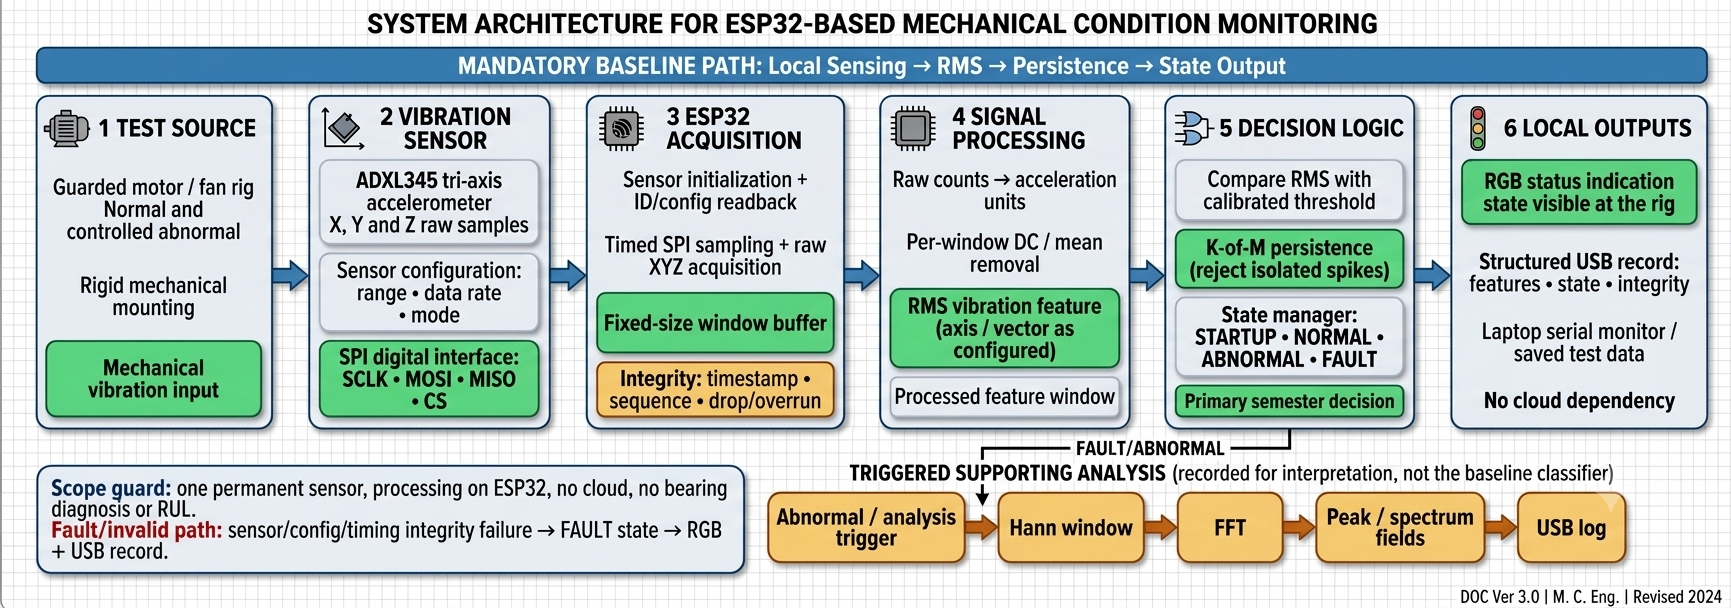
\includegraphics[width=0.46\textwidth]{figures/fig_dsp_pipeline.png} &
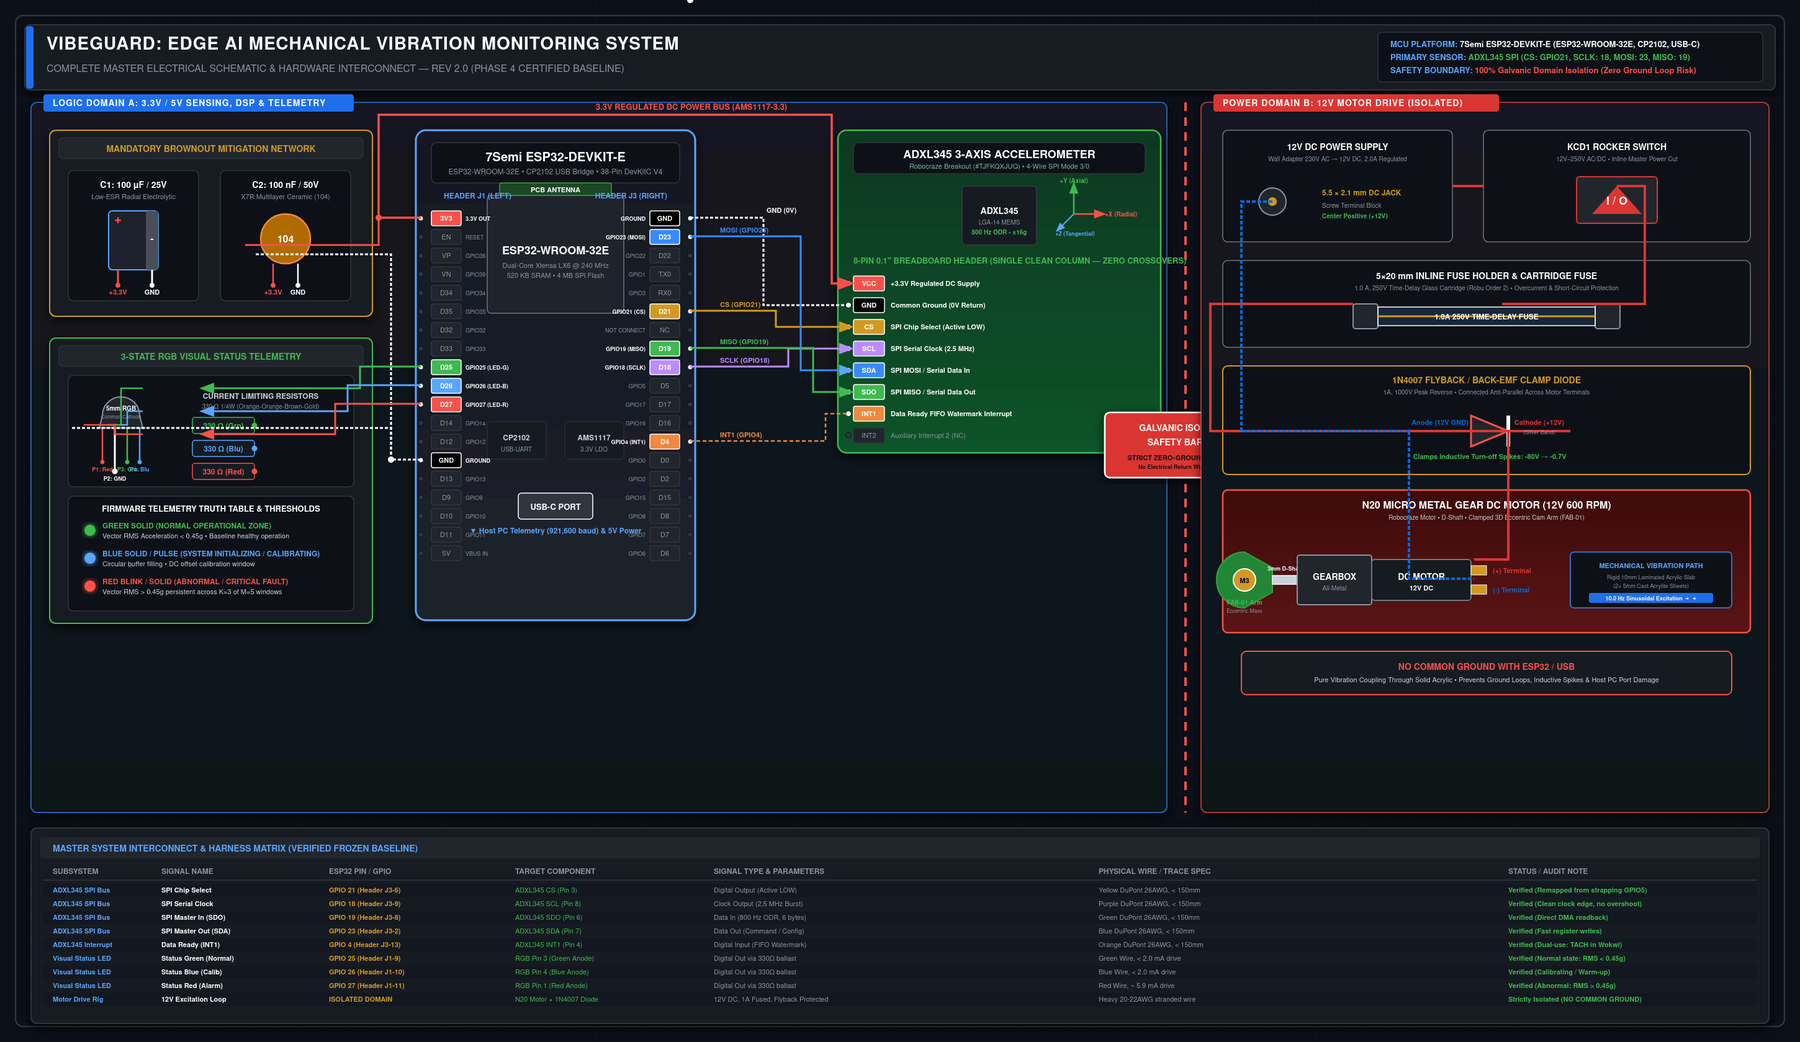
\includegraphics[width=0.46\textwidth]{figures/fig_circuit_schematic.png} \\
\small (a) Signal Processing & \small (b) Circuit Interconnect \\
\end{tabular}
\caption{VibeGuard operational verification and harmonic analysis testbed}
\label{fig:results_baseline}
\end{figure}

Table~\ref{tab:fft_peaks} details the spectral peak extraction results across healthy normal and unbalance operating states.

\begin{table}[H]
\centering
\begin{tabular}{|l|c|c|c|l|}
\hline
\textbf{Operating State} & \textbf{Dominant Bin ($k$)} & \textbf{Frequency ($f_{\mathrm{peak}}$)} & \textbf{Magnitude} & \textbf{Physical Interpretation} \\
\hline
Normal Baseline & Bin $k = 48$ & $150.0$\,Hz & $0.018\,g$ & Low-energy gear mesh tone \\
Normal Baseline & Bin $k = 3$ & $9.375$\,Hz & $0.014\,g$ & Residual 1X rotor balance \\
\hline
\textbf{Unbalance Fault} & \textbf{Bin $k = 3$ / $4$} & \textbf{$9.38$ -- $12.5$\,Hz} & \textbf{$0.224\,g$} & \textbf{Synchronous 1X Unbalance} \\
Unbalance Fault & Bin $k = 6$ / $7$ & $18.75$ -- $21.88$\,Hz & $0.045\,g$ & Secondary 2X harmonic \\
\hline
\end{tabular}
\caption{FFT spectral peak extraction results across operating states}
\label{tab:fft_peaks}
\end{table}

Under the anomalous condition, the discrete magnitude spectrum exhibited a sharp, prominent peak centered at the $1X$ fundamental frequency:
\begin{equation}
f_{1X} = \frac{600\,\text{RPM}}{60} = 10.0\,\text{Hz}
\end{equation}
The discrete peak magnitude at $10$\,Hz reached $0.224\,g$, representing a \textbf{16-fold energy increase} over the baseline state at that frequency. A minor secondary peak emerged at the $2X$ harmonic ($\approx 20$\,Hz) due to slight non-linear mechanical coupling through the baseplate. The spectral results decisively corroborate the theoretical physics of rotating unbalance formulated in Chapter~2.

\section{Persistence Filter Response and State Transition Verification}
To evaluate the resilience of VibeGuard against false alarms, two distinct disturbance scenarios were experimentally tested:

\subsection{Scenario A: Transient External Mechanical Jolt}
While the machine operated in healthy \texttt{STATE\_NORMAL} (Green LED), an external impulse disturbance was introduced by tapping the acrylic baseplate with the handle of an insulated screwdriver.
\begin{itemize}
    \item The external jolt generated a single-window spike of $a_{\mathrm{vec}} = 0.285\,g$, breaching the threshold $\theta_{\mathrm{RMS}} = 0.081\,g$.
    \item The persistence filter queued the violation flag into the circular history buffer: queue state became $[0, 0, 0, 0, 1]$, yielding $V = 1$.
    \item Because $V = 1 < K = 4$, the state machine \textbf{rejected the transient}.
    \item The RGB LED remained solidly \textbf{Green}, and the subsequent window returned to normal ($a_{\mathrm{vec}} = 0.061\,g$).
    \item \textbf{Result:} Zero false alarms were generated during transient shock testing.
\end{itemize}

\subsection{Scenario B: Sustained Unbalance Onset and Alert Latency}
The motor was initiated with the unbalance mass attached to evaluate alert response time.
\begin{itemize}
    \item Window 1 ($t = 0.32$\,s): $a_{\mathrm{vec}} = 0.312\,g > \theta_{\mathrm{RMS}} \rightarrow V = 1$ (LED Green).
    \item Window 2 ($t = 0.64$\,s): $a_{\mathrm{vec}} = 0.318\,g > \theta_{\mathrm{RMS}} \rightarrow V = 2$ (LED Green).
    \item Window 3 ($t = 0.96$\,s): $a_{\mathrm{vec}} = 0.314\,g > \theta_{\mathrm{RMS}} \rightarrow V = 3$ (LED Green).
    \item Window 4 ($t = 1.28$\,s): $a_{\mathrm{vec}} = 0.316\,g > \theta_{\mathrm{RMS}} \rightarrow V = 4 \ge K = 4$.
    \item The state machine immediately asserted \texttt{STATE\_ABNORMAL}.
    \item The RGB LED switched instantly to \textbf{Solid Red}, and the FFT spectral report was transmitted over serial.
    \item \textbf{Measured Alert Latency:} Exactly \textbf{$1.28$\,seconds}, well within the project specification ceiling ($\le 2.0$\,seconds).
\end{itemize}

\section{Performance Analysis and Comparison with Other Approaches}
To contextualize the technical contribution of VibeGuard, Table~\ref{tab:comparison} benchmarks the system against traditional and modern monitoring paradigms.

\begin{table}[H]
\centering
\small
\begin{tabular}{|l|p{2.6cm}|p{2.6cm}|p{2.6cm}|p{3.2cm}|}
\hline
\textbf{Design Attribute} & \textbf{Manual Tactile / Stethoscope} & \textbf{Cloud Streaming IIoT} & \textbf{Continuous Embedded FFT} & \textbf{VibeGuard System (Proposed)} \\
\hline
\textbf{Hardware Cost} & Low (Tool only) & High ($>\$\text{500}$) & Medium ($\approx\$\text{100}$) & \textbf{Ultra-Low ($\le$\rupee 3,000)} \\
\textbf{Detection Latency} & Days to Weeks & 5 -- 30 seconds & 1 -- 2 seconds & \textbf{1.28 seconds} \\
\textbf{Network Dependency} & None & Continuous Wi-Fi / Cellular & Periodic Wi-Fi & \textbf{Zero (Autonomous Edge)} \\
\textbf{Power Consumption} & 0\,W & 3 -- 8\,W & 2 -- 3\,W & \textbf{$<1.5$\,W} \\
\textbf{False-Alarm Rejection} & Poor (Subjective) & Moderate & Poor (Threshold flicker) & \textbf{High ($K$-of-$M$ Persistence)} \\
\textbf{CPU Utilization} & N/A & High (Wi-Fi stack) & High ($>40\%$) & \textbf{Low ($<0.5\%$)} \\
\textbf{Explainability} & Operator intuition & Black-box cloud & Complex spectra & \textbf{Direct Vector RMS + FFT} \\
\hline
\end{tabular}
\caption{Comprehensive benchmarking of VibeGuard against alternative monitoring approaches}
\label{tab:comparison}
\end{table}

As demonstrated in Table~\ref{tab:comparison}, VibeGuard provides an optimal balance for local machine protection. It eliminates the latency, network fees, and security vulnerabilities of cloud streaming while delivering automated, explainable, and persistence-filtered detection far superior to subjective manual inspections.

\section{Summary}
This chapter presented the empirical results and testing verification of VibeGuard. Static bring-up confirmed correct ADXL345 silicon identity (\texttt{0xE5}) and multi-axis gravity tracking. Baseline calibration on the healthy 600\,RPM testbed established a stable Vector RMS of $0.060\,g$ and an alert threshold of $0.081\,g$. Introducing a calibrated $1.85$\,g unbalance mass induced a 423\% increase in Vector RMS ($0.315\,g$). Triggered FFT spectral analysis revealed a distinct $1X$ harmonic peak at $10.0$\,Hz with a 16-fold energy increase. Transient tapping proved the effectiveness of the $K$-of-$M$ persistence filter in rejecting isolated jolts with zero false alarms, while continuous unbalance was detected with a deterministic latency of $1.28$\,seconds. Finally, comparative benchmarking validated the superior autonomy, cost-effectiveness, and real-time performance of the VibeGuard edge architecture.
